
\section{Weierstrass Theorem}  
To approximate any continuous function, a very simple idea is to approximate the function in a polynomial space. 
An important property of this space is that polynomials can approximate any reasonable function!
\begin{itemize}
\item $P_n(\mathbb{R}^d)$ is dense in $C(\Omega)$ [Weierstrass theorem]
\item $P_n(\mathbb{R}^d)$ is dense in all Sobolev spaces: $L^2(\Omega), W^{m,p}(\Omega), \ldots$
\end{itemize}

\begin{theorem}
Let $\Omega\subset R^n$ be a  closed and bounded set. Given any continuous function $f(x)$ on $\Omega$, there exists a sequence of polynomials $\{p_n(x)\}$ such 
that 
\begin{equation}
\displaystyle \lim_{n\rightarrow \infty} \max_{x\in \Omega}|f(x)-p_n(x)|=0
\end{equation}
\end{theorem}
\begin{proof}
Let us first give the proof for $d=1$ and $\Omega=[0,1]$. Given $f:[0,1]\rightarrow R$ be a  continuous function. 

Let
\begin{equation}
\tilde f(x)=f(x)-l(x)
\end{equation}
where $l(x)=f(0)+x(f(1)-f(0))$.
Then $\tilde f(0)=\tilde f(1)=0$. Noting that $l(x)$ is a linear function, hence without lose of generality, we can only consider the 
case $f:[0,1]\rightarrow R$ with $f(0)=f(1)=0$. 
Since $f$ is continuous on the closed interval $[0,1]$, then $f$ is uniformly continuous on $[0,1]$.

First we extend $f$ to be zero outside of $[0,1]$ and obtain $f: R\rightarrow R$, then it is obviously that $f$ is still uniformly continuous. 

Next for $0\le x\le 1$, we construct
\begin{equation}
p_n(x)=\int_{-1}^1f(x+t)Q_n(t)dt=\int_{-x}^{1-x}f(x+t)Q_n(t)dt=\int_{0}^{1}f(t)Q_n(t-x)dt
\end{equation} 
where $Q_n(x)=c_n(1-x^2)^n$ and 
\begin{equation}\label{intq}
\int_{-1}^1 Q_n(x) dx=1.
\end{equation} 
Thus $\{p_n(x)\}$ is a sequence of polynomials. 

Since 
\begin{align}
\int_{-1}^1 (1-x^2)^n dx&=2\int_{0}^1 (1-x^2)^n dx=  2\int_{0}^1 (1-x)^n(1+x)^n dx\\ 
&\ge 2\int_{0}^1 (1-x)^n dx=\frac{2}{n+1}> \frac{1}{n}.
\end{align}
Combing with $\int_{-1}^1 Q_n(x) dx=1$, we obtain $c_n< n$ implying that for any $\delta>0$
 \begin{equation}\label{qest}
 0\le Q_n(x)\le n(1-\delta^2)^n \quad (\delta\le |x|\le 1),
 \end{equation}
so that $Q_n\rightarrow 0$ uniformly in $\delta\le |x|\le 1$ as $n\rightarrow \infty$. 

Given any $\epsilon >0$, since $f$ in uniformly continuous, there exists $\delta>0$ such that for any $|y-x|<\delta$, we have 
\begin{equation}\label{fcont}
|f(y)-f(x)|< \frac{\epsilon}{2}.
\end{equation}
Finally, let $M=\max |f(x)|$, using \eqref{fcont}, \eqref{intq} and \eqref{qest}, we have 
\begin{align}
\big| p_n(x)-f(x)\big|&=\big|\int_{-1}^1(f(x+t)-f(t))Q_n(t)dt\big|\le \int_{-1}^1 \big| f(x+t)-f(t)\big| Q_n(t)dt\\
&\le 2M \int_{-1}^{-\delta} Q_n(t)dt+ \frac{\epsilon}{2}\int_{-\delta}^{\delta} Q_n(t)dt+ 2M\int_{\delta}^1 Q_n(t)dt\\
&\le 4M n(1-\delta^2)^n + \frac{\epsilon}{2}< \epsilon
\end{align}
for all large enough $n$, which proves the theorem. 

The above proof generalize the high dimensional case easily.   We
consider the case that
$$
\Omega=[0,1]^d.
$$
By extension and using cut off function,  W.L.O.G.  that we assume
that $f=0$ on the boundary of $\Omega$ and we then extending this
function to be zero outside of $\Omega$.  

Let us consider the special polynomial functions
\begin{equation}
  \label{Qn}
Q_n(x)=c_n\prod_{k=1}^d(1-x_k^2)  
\end{equation}
Similar proof can then be applied. 
\end{proof}























 
\subsection{Curse of dimensionality}
Number of coefficients for polynomial space $P_n(\mathbb{R}^d)$  is
$$
	N = \binom{d+n}{n} = \frac{(n+d)!}{d!n!}.
$$
For example $n = 100$:
		\begin{table}
			\centering
			\begin{tabular}{|c|c|c|c|}
				\hline
				$d = $&  $2$ &  $4$ & $8$\\
				\hline
				$N=$  & $5\times10^3$ & $4.6\times10^6$  & $3.5\times10^{11}$ 	\\
				\hline
			\end{tabular}
		\end{table}
As the this table shows, the dimension of the polynomial space $P_n(\mathbb{R}^d)$   increases rapidly as the degree $n$ increases. This leads to an extremely large space therefore very expensive to approximate functions in polynomial spaces in high dimensions.
\subsection{Runge's phenomenon}
A natural way to approximate a given function on any interval $[a,b]$ is to use an $n$-degree polynomial $p_n(x)$ by $n+1$ equispaced  points, namely
$$
x_i=a+{b-a\over n},\quad i=0,1,2,\cdots,n.
$$
By Weierstrass' theorem, we expect a more accurate reconstruction of $f(x)$ by using more points. But this is not always true as shown in the following example. 
%Consider the case where one desires to interpolate through $n+1$ equispaced points of a function $f(x)$ using the n-degree polynomial $p_n(x)$ that passes through those points. Naturally, one might expect from Weierstrass' theorem that using more points would lead to a more accurate reconstruction of $f(x)$. However, this particular set of polynomial functions $p_n(x)$ is not guaranteed to have the property of uniform convergence; the theorem only states that a set of polynomial functions exists, without providing a general method of finding one.

Consider the Runge function (a scaled version of the Witch of Agnesi)
$$ 
f(x)=\frac{1}{1+25x^{2}}.
$$
Runge found that if this function is interpolated at equidistant points $x_i$ between $-1$ and $1$ such that:
$$
x_{i}={\frac{2i}{n}}-1,\quad i\in \left\{0,1,\dots ,n\right\}
$$
with a polynomial $p_n(x)$ of degree $\leq n$, the resulting interpolation oscillates toward the ends of the interval, i.e. close to $-1$ and $1$. It can even be proven that the interpolation error increases (without bound) when the degree of the polynomial is increased:

$$\lim_{{n\rightarrow \infty }}\left(\max_{{-1\leq x\leq 1}}|f(x)-p_{n}(x)|\right)=+\infty.$$
This shows that high-degree polynomial interpolation at equidistant points can be troublesome.

\begin{figure}
	\begin{center}
		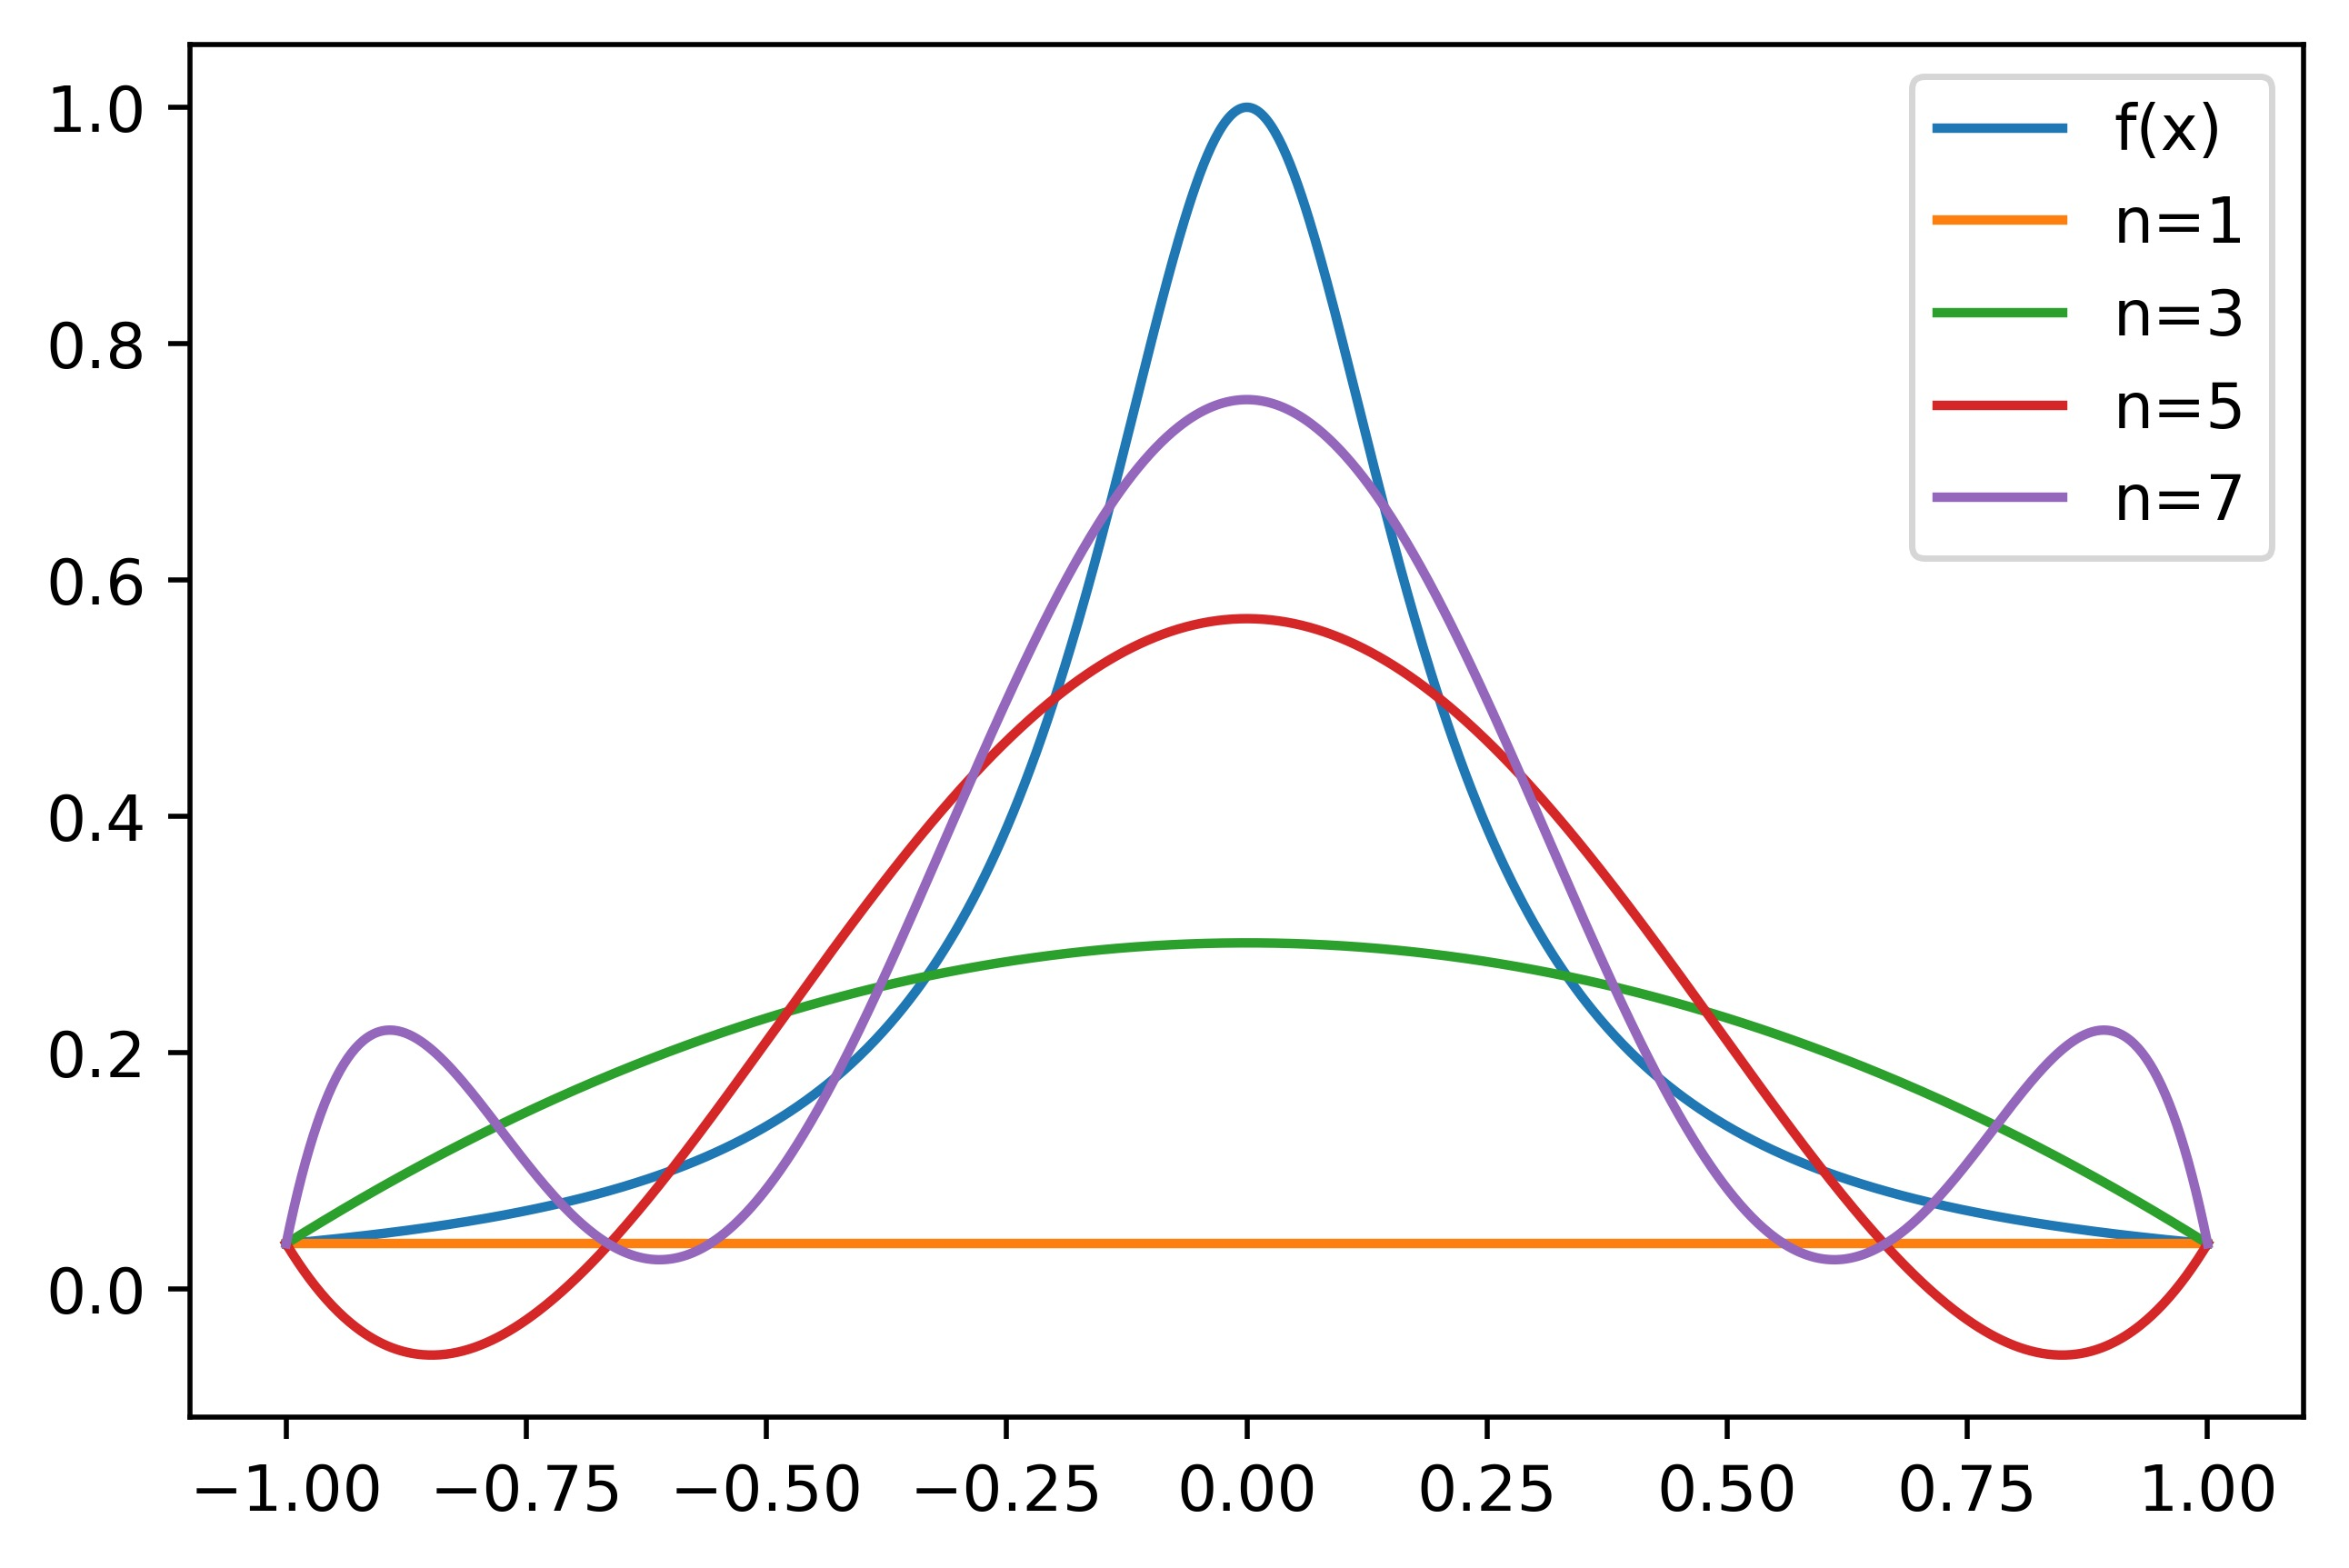
\includegraphics[scale=0.1]{6DL/pic/Runge.jpeg}
		\caption{Runge's phenomenon: Runge function $f(x)=\frac{1}{1+25x^{2}}$ and its polynomial interpolation $p_n(x)$.}
	\end{center}
\end{figure}

The experiment shows that  the polynomials $p_n(x)$ produced in this manner may in fact diverge away from $f(x)$ as $n$ increases. This typically occurs in an oscillating pattern that magnifies near the ends of the interpolation points. This phenomenon is attributed to Runge.

Thus, this particular set of polynomial functions $p_n(x)$ is not guaranteed to have the property of uniform convergence. In other words, Weierstrass' theorem guarantees the existence of the polynomial functions, but how to find such polynomials is not provided.

\section{Fourier transform and Fourier series}
We make use of the theory of tempered distributions (see
\cite{strichartz2003guide} for an introduction)
and we begin by collecting some results of independent interest, which
will also be important later. 
\subsection{Fourier transform}
Before studying the Fourier transform, we first consider Schwartz space which is defined below.
\begin{definition} \label{def:schwarz}
The Schwartz space $\mathcal{S}\left(\mathbb{R}^{n}\right)$ is the topological vector space of functions $f: \mathbb{R}^{n} \rightarrow \mathbb{C}$ such that $f \in C^{\infty}\left(\mathbb{R}^{n}\right)$ and
$$
x^{\alpha} \partial^{\beta} f(x) \rightarrow 0 \quad \text { as }|x| \rightarrow \infty
$$
for every pair of multi-indices $\alpha, \beta \in \mathbb{N}_{0}^{n} .$ For $\alpha, \beta \in \mathbb{N}_{0}^{n}$ and $f \in \mathcal{S}\left(\mathbb{R}^{n}\right)$ let
(5.10)
$$
\|f\|_{\alpha, \beta}=\sup _{\mathbb{R}^{n}}\left|x^{\alpha} \partial^{\beta} f\right|
$$
A sequence of functions $\left\{f_{k}: k \in \mathbb{N}\right\}$ converges to a function $f$ in $\mathcal{S}\left(\mathbb{R}^{n}\right)$ if
$$
\left\|f_{n}-f\right\|_{\alpha, \beta} \rightarrow 0 \quad \text { as } k \rightarrow \infty
$$
for every $\alpha, \beta \in \mathbb{N}_{0}^{n}$.
\end{definition}
The Schwartz space consists of smooth functions whose derivatives and the function itself decay at infinity faster than any power. Schwartz functions are rapidly decreasing. When there is no ambiguity, we will write $\mathcal{S}\left(\mathbb{R}^{n}\right)$ as $\mathcal{S}$.
Roughly speaking, tempered distributions grow no faster than a polynomial at infinity.

\begin{definition}
A tempered distribution $T$ on $\mathbb{R}^{n}$ is a continuous linear functional $T: \mathcal{S}\left(\mathbb{R}^{n}\right) \rightarrow \mathbb{C} .$ The topological vector space of tempered distributions is denoted by $\mathcal{S}^{\prime}\left(\mathbb{R}^{n}\right)$ or $\mathcal{S}^{\prime} .$ If $\langle T, f\rangle$ denotes the value of $T \in \mathcal{S}^{\prime}$ acting on $f \in \mathcal{S}$
then a sequence $\left\{T_{k}\right\}$ converges to $T$ in $\mathcal{S}^{\prime}$, written $T_{k} \rightarrow T$, if
$$
\left\langle T_{k}, f\right\rangle \rightarrow\langle T, f\rangle
$$
for every $f \in \mathcal{S}$.
\end{definition}
Since $\mathcal{D} \subset \mathcal{S}$ is densely and continuously imbedded, we have $\mathcal{S}^{\prime} \subset \mathcal{D}^{\prime} .$ Moreover, a distribution $T \in \mathcal{D}^{\prime}$ extends uniquely to a tempered distribution $T \in \mathcal{S}^{\prime}$ if and only if it is continuous on $\mathcal{D}$ with respect to the topology on $\mathcal{S}$. Every function $f \in L_{\text {loc }}^{1}$ defines a regular distribution $T_{f} \in \mathcal{D}^{\prime}$ by
$$
\left\langle T_{f}, \phi\right\rangle=\int f \phi d x \quad \text { for all } \phi \in \mathcal{D}.
$$
If $|f| \leq p$ is bounded by some polynomial $p,$ then $T_{f}$ extends to a tempered distribution $T_{f} \in \mathcal{S}^{\prime}$, but this is not the case for functions $f$ that grow too rapidly at infinity.

The Schwartz space is a natural one to use for the Fourier transform. Differentiation and multiplication exchange roles under the Fourier transform and therefore so do the properties of smoothness and rapid decrease. As a result, the Fourier transform is an automorphism of the Schwartz space. By duality, the Fourier transform is also an automorphism of the space of tempered distributions.

\begin{definition}\label{def:fourier1}
The Fourier transform of a function $f \in \mathcal{S}\left(\mathbb{R}^{n}\right)$ is the function $\hat{f}: \mathbb{R}^{n} \rightarrow \mathbb{C}$ defined by 
$$
\hat{f}(\omega)= \int f(x) e^{-2 \pi i\omega \cdot x} d x.
$$
The inverse Fourier transform of $f$ is the function $\check{f}: \mathbb{R}^{n} \rightarrow \mathbb{C}$ defined by
$$
\check{f}(x)=\int f(\omega) e^{2 \pi i\omega \cdot x} d k.
$$
\end{definition}

\begin{definition}\label{def:fourier2}
The Fourier transform of a tempered distribution $f \in \mathcal{S}'$ is  defined by 
$$
\langle \hat{f}, \phi\rangle = \langle f, \hat \phi\rangle,\quad \forall \phi\in \mathcal{S}.
$$ 
\end{definition}

The support of a continuous function $f$ is the closure  of the set $\{x\in \mathbb{R}: f(x)\neq 0\}$.
\begin{properties}
The Fourier transform has the following properties
\begin{enumerate}
\item If $f\in \mathcal{S}'$ and the support of $\hat f$ is $\{0\}$, then $f$ is a polynomial.
\item If $f\in \mathcal{S}'$ and the support of $\hat f$ is a single point $\{a\}$, then $f(x)=e^{2\pi iax}P(x)$, where $P(x)$ is a polynomial.
\end{enumerate}
\end{properties}







\subsection{Poisson summation formula}
% Qingguo put the Poisson summation formula here in this file:  statement and sketch of proof

\begin{theorem}
Let $f \in L^{1}(\mathbb{R})$ and $f$ is continuous. Then we have for almost all $(x, \omega ) \in \mathbb{R} \times \hat{\mathbb{R}}$ that
$$
T \sum_{n \in \mathbb{Z}} f(x+n T) e^{-2 \pi i \omega (x+n T)}=\sum_{n \in \mathbb{Z}} \hat{f}\left(\omega +\frac{n}{T}\right) e^{2 \pi i n x / T}
$$
where both sides converge absolutely.

In addition,  let $\Lambda$ be the lattice in $\mathbb{R}^{d}$ consisting of points with integer coordinates. 
For a function $f$ in $L^{1}\left(\mathbb{R}^{d}\right)$ and $f$ is continuous, we have 
$$
\sum_{\omega  \in \Lambda} f(x+\omega )=\sum_{\nu \in \Lambda} \hat{f}(\omega ) e^{2 \pi i x \cdot \omega }.
$$
where both series converge absolutely and uniformly on $\Lambda$. 
\end{theorem} 

\begin{proof}
We just give a proof of a simple case that $f: \mathbb{R} \rightarrow \mathbb{C}$ is a Schwarz function (see Definition \ref{def:schwarz}).
Let:
$$
F(x)=\sum_{n \in \mathbb{Z}} f(x+n).
$$
Then $F(x)$ is 1-periodic (because of absolute convergence), and has Fourier coefficients:
$$
\begin{aligned}
\hat{F}_{\omega } &=\int_{0}^{1} \sum_{n \in \mathbb{Z}} f(x+n) e^{-2 \pi i \omega x} \mathrm{~d} x \\
&=\sum_{n \in \mathbb{Z}} \int_{0}^{1} f(x+n) e^{-2 \pi i \omega  x} \mathrm{~d} x \quad \text { because } f \text { is Schwarz, so convergence is uniform}\\
&=\sum_{n \in \mathbb{Z}} \int_{n}^{n+1} f(x) e^{-2 \pi i\omega  x} \mathrm{~d} x \\
&=\int_{\mathbb{R}} f(x) e^{-2 \pi i \omega  x} \mathrm{~d} x\\
&=\hat{f}(k)\\
\end{aligned}
$$
 where $\hat{f}$ is the Fourier transform of $f$.
 

Therefore by the definition of the Fourier series of $f:$
$$
F(x) =\sum_{\omega  \in \mathbb{Z}} \hat{f}(k) e^{2\pi i \omega x}.
$$
Choosing $x=0$ in this formula:
$$
\sum_{n \in \mathbb{Z}} f(n)=\sum_{\omega  \in \mathbb{Z}} \hat{f}(\omega )
$$
as required.
\end{proof}






\subsection{A special cut-off function}
Let us first state the following simple result that can be obtained by following a calculation given in Section 3 of \cite{johnson2015saddle}. 
\begin{lemma} Given $\alpha>1$, consider
 \begin{equation}\label{alpha-g}
  g(t) = \begin{cases} 
      e^{-(1-t^2)^{1 - \alpha}} & t\in (-1,1) \\
      0 & \text{otherwise}.
   \end{cases}
 \end{equation}
then there is a constant $c_\alpha$ such that
 \begin{equation}\label{eq_181}
  |\hat{g}(\omega )|\lesssim e^{-c_\alpha|\omega |^{1-\alpha^{-1}}},
 \end{equation}
\end{lemma}
\begin{proof}
Consider the asymptotic behavior of the Fourier transform
$$
F(\omega )=\int_{-\infty}^{\infty} g(t) e^{2\pi i \omega  t} dt=2 \operatorname{Re} \int_{0}^{1} e^{2\pi i \omega  t- (1-t^{2})^{1-\alpha}} dt
$$
for $|\operatorname{Re} \omega | \gg 1.$ (Without loss of generality, we can restrict ourselves to real $\omega  \geq 0$).  
With a change of variable $x=1-t$,
$$
F(\omega )=2 \operatorname{Re} \int_{0}^{1} e^{f(x)} dx
$$
with 
$
f(x)=2\pi i \omega  - 2\pi i \omega   x- (2x-x^2)^{1-\alpha}\approx \tilde f(x)+O\left(x^{2-\alpha}\right)
$
and 
$$
\tilde f(x) = 2\pi i \omega  - 2\pi i \omega    x - (2 x)^{1-\alpha}.
$$
The saddle point is the $x=x_0$ where $f'(x_0)=0$. Since
$
\tilde f'(x)=-2\pi i \omega  + (\alpha-1)2^{1-\alpha} x^{-\alpha},
$
$$
x_{0} \approx \tilde x_0=\left (2^{-\alpha} (\alpha-1) / i \omega \pi \right )^{1 / \alpha} \sim \omega ^{-1 / \alpha}.
$$
Therefore $\tilde f(\tilde x_{0}) \sim \omega ^{(\alpha-1) / \alpha}$ asymptotically. The second derivative is 
$$
\tilde f'' (\tilde x_{0} )=-2^{1-\alpha}  \alpha(\alpha-1) \tilde x_{0}^{-\alpha-1}=-i^{(\alpha+1) / \alpha} 2 A \omega ^{(\alpha+1)/\alpha},
$$
where
$$
A=2\alpha  (\alpha-1)^{-1/\alpha}\pi^{(\alpha+1)/\alpha}.
$$
Now,
\begin{equation}
\begin{split}
\tilde f(x)\approx &\tilde f(\tilde x_0) + {\tilde f''(\tilde x_0)\over 2} (x-\tilde x_0)^2
\\
=&2\pi i \omega  - (\alpha - 1)^{1\over \alpha}(i\omega \pi )^{\alpha -1\over \alpha}  - (\alpha - 1)^{1-\alpha\over \alpha} (i\omega \pi )^{\alpha -1\over \alpha}
\\
&-i^{(\alpha+1) / \alpha} A \omega ^{(\alpha+1)/\alpha}(x- 2^{-1}(\alpha - 1)^{-{1\over \alpha}}(i\omega \pi )^{-{1\over \alpha}} )^2.
\end{split}
\end{equation} 
Choose a contour $x=i^{-1 / \alpha}u$, in which case  
$$
\tilde f(x) \approx \tilde f(\tilde x_{0}) -i^{(\alpha-1) / \alpha} A \omega ^{(\alpha+1) / \alpha}\left(u-u_{0}\right)^{2},
$$
which is a path of descent so we can perform a Gaussian integral. 

Recall that the integral of 
\begin{equation}\label{gaussInt}
\int_{-\infty}^{\infty} e^{-a u^{2}} d u=\sqrt{\pi / a}
\end{equation}
as long as Re$a>0,$ which is true here. Note also that, in the limit as $\omega $ becomes large, the integrand becomes zero except close to $u=\sqrt{1 / 2 \omega },$ so we can neglect the rest of the contour and treat the integral over $u$ as going from $-\infty$ to $\infty$. (Thankfully, the width of the Gaussian $\Delta u \sim \omega ^{-3 / 4}$ goes to zero faster than the location of the maximum $u_{0} \sim \omega ^{-1 / 2},$ so we don't have to worry about the $u=0$ origin). Also note that the change of variables from $x$ to $u$ gives us the Jacobian factor for 
$$dx=i^{-1 / \alpha}d u.$$ 
Thus, when all is said and done, we obtain the exact asymptotic form of the Fourier integral for $\omega  \gg 1$: 
\begin{equation}
\begin{split}
F(\omega ) \approx &2 \operatorname{Re}\int_{0}^{1} e^{\tilde f(\tilde x_0) - i^{(\alpha-1) / \alpha} A \omega ^{(\alpha+1) / \alpha}\left(u-u_{0}\right)^{2}} dx
\\
=&2 \operatorname{Re} e^{\tilde f(\tilde x_0)} i^{-1 / \alpha} \int_{-\infty}^{\infty} e^{- i^{(\alpha-1) \over  \alpha} A \omega ^{(\alpha+1) / \alpha}\left(u-u_{0}\right)^{2}} du
\\
=&2 \operatorname{Re} e^{\tilde f(\tilde x_0)} \pi^{1/2}i^{-1 / \alpha}  i^{(1-\alpha) \over  2\alpha} A^{-1/2} \omega ^{-(\alpha+1) / 2\alpha}\qquad \text{ by \eqref{gaussInt}} 
\\
=&2 \operatorname{Re}\left[\sqrt{\frac{\pi}{(i \omega )^{(\alpha+1) / \alpha} A}} e^{\tilde f(\tilde x_0)}\right]
\\
\approx &2 \operatorname{Re}\left[\sqrt{\frac{\pi}{(i \omega )^{(\alpha+1) / \alpha} A}} e^{ 2\pi i \omega - 2\pi i \omega  \tilde x_{0}- \left[\left(2-\tilde x_{0}\right) \tilde x_{0}\right]^{1-\alpha}}\right]
\end{split}
\end{equation}  
with $x_{0}$ and $A$ given above.  Notice that $ \tilde x_0\sim \omega ^{-1 / \alpha}$. Thus,
$$
|F(\omega ) | \approx  e^{-c_\alpha|\omega |^{1-\alpha^{-1}}}.
$$
\end{proof}

\subsection{Fourier transform of polynomials}
We begin by noting that an activation
function $\sigma$, which satisfies a polynomial growth condition
$|\sigma(x)| \leq C(1 + |x|)^n$ for some constants $C$ and $n$, is a
tempered distribution. As a result, we make this assumption on our
activation functions in the following theorems. We briefly note that
this condition is sufficient, but not necessary (for instance an
integrable function need not satisfy a pointwise polynomial growth
bound) for $\sigma$ to be represent a tempered distribution.

 We begin by studying the convolution of $\sigma$ with a Gaussian mollifier. Let $\eta$ be a Gaussian mollifier
 \begin{equation}
  \eta(x) = \frac{1}{\sqrt{\pi}}e^{-x^2}.
 \end{equation}
Set $\eta_\epsilon=\frac{1}{\epsilon}\eta(\frac{x}{\epsilon})$. Then consider 
\begin{equation}
\label{sigma-epsilon}
\sigma_{\epsilon}(x):=\sigma\ast{\eta_\epsilon}(x)=\int_{\mathbb{R}}\sigma(x-y){\eta_\epsilon}(y)dy
\end{equation}
for a given activation function $\sigma$.
It is clear that $\sigma_{\epsilon}\in C^\infty(\mathbb{R})$. Moreover, by considering the Fourier transform (as a tempered
distribution) we see that
\begin{equation}\label{eq_278}
 \hat{\sigma}_{\epsilon} = \hat{\sigma}\hat{\eta}_{\epsilon} = \hat{\sigma}\eta_{\epsilon^{-1}}.
\end{equation} 


We begin by stating a lemma which characterizes the set of polynomials in terms of their
 Fourier transform.
\begin{lemma}\label{polynomial_lemma} Given a tempered distribution
  $\sigma$,  the following statements are equivalent:
\begin{enumerate}
\item $\sigma$ is a polynomial 
\item $\sigma_\epsilon$ given by \eqref{sigma-epsilon} is a polynomial for any
  $\epsilon>0$. 
\item $\text{\normalfont supp}(\hat{\sigma})\subset \{0\}$. 
\end{enumerate}
\end{lemma}
\begin{proof}
  We begin by proving that (3) and (1) are equivalent.  This follows
  from a characterization of distributions supported at a single point
  (see \cite{strichartz2003guide}, section 6.3). In particular, a
  distribution supported at $0$ must be a finite linear combination of
  Dirac masses and their derivatives.  In particular, if
  $\hat{\sigma}$ is supported at $0$, then
  \begin{equation}
   \hat{\sigma} = \displaystyle\sum_{i=1}^n a_i\delta^{(i)}.
  \end{equation}
  Taking the inverse Fourier transform and noting that the inverse
  Fourier transform of $\delta^{(i)}$ is $c_ix^i$, we see that
  $\sigma$ is a polynomial. This shows that (3) implies (1), for the
  converse we simply take the Fourier transform of a polynomial and
  note that it is a finite linear combination of Dirac masses and
  their derivatives.
  
  Finally, we prove the equivalence of (2) and (3). For this it
  suffices to show that $\hat{\sigma}$ is supported at $0$ iff
  $\hat{\sigma}_\epsilon$ is supported at $0$. This follows from
  equation \ref{eq_278} and the fact that $\eta_{\epsilon^{-1}}$ is
  nowhere vanishing.
\end{proof}

As an application of Lemma \ref{polynomial_lemma}, we give a
simple proof of the result in the next section.   

